\documentclass[12pt, oneside]{article} 
\usepackage{amsmath, amsthm, amssymb, calrsfs, wasysym, verbatim, bbm, color, colortbl, graphicx, geometry, fancyhdr, url, multirow, hyperref, titlesec, tabularx, spreadtab, pgf-pie, array, longtable, caption, float, subcaption, listings, comment}
\usepackage[italian]{babel}

\geometry{tmargin=.75in, bmargin=.75in, lmargin=.75in, rmargin = .75in}

% opzioni listing
\definecolor{codegreen}{rgb}{0,0.6,0}
\definecolor{codegray}{rgb}{0.5,0.5,0.5}
\definecolor{codepurple}{rgb}{0.58,0,0.82}
\definecolor{backcolour}{rgb}{0.95,0.95,0.92}

\lstdefinestyle{mystyle}{
    backgroundcolor=\color{backcolour},   
    commentstyle=\color{codegreen},
    keywordstyle=\color{magenta},
    numberstyle=\tiny\color{codegray},
    stringstyle=\color{codepurple},
    basicstyle=\ttfamily\footnotesize,
    breakatwhitespace=false,         
    breaklines=true,                 
    captionpos=b,                    
    keepspaces=true,                 
    numbers=left,                    
    numbersep=5pt,                  
    showspaces=false,                
    showstringspaces=false,
    showtabs=false,                  
    tabsize=2
}

\lstset{style=mystyle}

\author{RAMtastic6}

%Intestazione
\pagestyle{fancy}
\fancyhf{}
\fancyhead[R]{Gruppo 14 RAMtastic6\\ramtastic6@gmail.com}
\fancyfoot[C]{\thepage}

% Linea intestazione
\renewcommand{\headrulewidth}{1pt} 

% Intestazione documento
\begin{document}
% Salta la prima pagina per l'intestazione
\thispagestyle{empty}
\title{Manuale Utente}
\maketitle
\begin{figure}[h]
  \centering
  
\includegraphics[scale=0.3]{logo.png}
\end{figure}
\begin{center}
    email: ramtastic6@gmail.com
\end{center}

% Informazioni sul documento
\section*{Informazioni sul documento} 
\begin{tabular}{ll}
Versione: & 1.0.0 \\
Redattori: &  Zaupa R. Basso L. Brotto D. Zambon M. Tonietto F.\\ 
Verificatori: & Zambon M. Tonietto F. Brotto D\\
Destinatari: & Vardanega T., Cardin R., Imola Informatica \\
Uso: & Esterno
\end{tabular}
\newpage

% Registro dei cambiamenti
\section*{Registro dei Cambiamenti - Changelog}
\begin{longtable}{|c|c|c|c|p{7cm}|}
\hline
\textbf{Versione} & \textbf{Data} & \textbf{Autore} & \textbf{Verificatore} & 
\textbf{Dettaglio} \\
\hline
v 1.0.0 & 2024-06-11 & Brotto D. & Brotto D. & Approvazione e validazione del documento \\
\hline
v 0.3.0 & 2024-06-08 & Tonietto F. & Brotto D & Stesura della sezione 4 relativa al "Supporto tecnico". \\
\hline
v 0.2.1 & 2024-06-08 & Tonietto F. & Brotto D & Stesura delle sezioni relative alla descrizione del funzionamento del $\textit{sistema}_G$ di notifica sia per l'utente base che per l'amministratore. \newline Stesura delle sezioni relative alla visualizzazione dell'elenco delle prenotazioni effettuate/ricevute e del relativo dettaglio sia per l'utente base che per l'amministratore. \\
\hline
v 0.2.0 & 2024-06-06 & Zambon M. & Tonietto F. & Stesura della sezione 3.2.5 \\
\hline
v 0.1.1 & 2024-06-05 & Zambon M. & Tonietto F. & Stesura della sezione 3.2.3 \\
\hline
v 0.1.0 & 2024-06-01 & Basso L. & Zambon M. & Stesura della sezione installazione (3.1.1). Stesura della sezione 3.2.1. \\
\hline
v 0.0.3 & 2024-05-31 & Brotto D. & Zambon M. & Stesura della sezione 3.2.2 e 3.2.4. \\
\hline
v 0.0.2 & 2024-05-21 & Basso L. & Zambon M. & Stesura della sezione 2 (requisiti). \\
\hline
v 0.0.1 & 2024-05-17 & Zaupa R. & Zambon M. & Prima versione, stesura della sezione "Introduzione" \\
\hline
\end{longtable}
\newpage

% Sommario
\tableofcontents
\newpage

% Introduzione
\section{Introduzione}
\subsection{Scopo del documento}
Il presente documento si propone di definire le metriche e le metodologie di controllo e misurazione necessarie per garantire la qualità del prodotto e del processo. In particolare, le metriche di valutazione del prodotto sono correlate ai requisiti e alle aspettative del fornitore.
Il Piano di Qualifica è concepito per essere dinamico ed incrementale, in particolar modo per quanto riguarda le metriche descritte e mira a fornire una valutazione il più obiettiva possibile di ciò che è stato realizzato.\\
Le procedure del Way of Working devono essere costantemente osservate e migliorate, al fine di garantire che il prodotto soddisfi le aspettative del cliente e mantenga gli standard di qualità richiesti. Eventuali termini tecnici sono definiti all'interno del documento "Glossario Tecnico".

\subsection{Riferimenti}
\subsubsection{Riferimenti normativi}
\begin{enumerate}
    \item Norme di Progetto
    \item Presentazione del capitolato d'appalto C3 - Progetto Easy Meal: \\ 
    \url{https://www.math.unipd.it/~tullio/IS-1/2023/Progetto/C3.pdf}
    \item Regolamento del progetto didattico: \\ 
    \url{https://www.math.unipd.it/~tullio/IS-1/2023/Dispense/PD2.pdf}
\end{enumerate}
\subsubsection{Riferimenti informativi}
\label{sec:rif_inf}
\begin{enumerate}
    \item Lezione \emph{"Progettazione software (T6)"} del corso di Ingegneria del software: \\
    \url{https://www.math.unipd.it/~tullio/IS-1/2023/Dispense/T6.pdf}
    \item Lezione \emph{"Qualità del software (T7)"} del corso di Ingegneria del software: \\
    \url{https://www.math.unipd.it/~tullio/IS-1/2023/Dispense/T7.pdf}
    \item Lezione \emph{"Qualità di processo (T8)"} del corso di Ingegneria del software: \\
    \url{https://www.math.unipd.it/~tullio/IS-1/2023/Dispense/T8.pdf}
    \item Lezione \emph{"Verifica e validazione: introduzione (T9)"} del corso di Ingegneria del software: \\
    \url{https://www.math.unipd.it/~tullio/IS-1/2023/Dispense/T9.pdf}
    \item Lezione \emph{"Verifica e validazione: analisi statica (T10)"} del corso di Ingegneria del software: \\
    \url{https://www.math.unipd.it/~tullio/IS-1/2023/Dispense/T10.pdf}
    \item Lezione \emph{"Verifica e validazione: analisi dinamica (T11)"} del corso di Ingegneria del software: \\
    \url{https://www.math.unipd.it/~tullio/IS-1/2023/Dispense/T11.pdf}
     \item Documento \emph{"Dichiarazione impegni v1.2"}: \\ \url{https://github.com/RAMtastic6/Project14/blob/main/documenti/CANDIDATURA/documento_impegni_v1.2.pdf}
     \item Metriche di progetto (\emph{Earned Value Analysis}):\\
     \url{https://it.wikipedia.org/wiki/Metriche_di_progetto}
\end{enumerate}
\subsection{Codifica delle metriche}
In questa sottosezione verranno definite le metriche che utilizzeremo, utilizzando un codice standardizzato.

Una metrica è identificata dal seguente formato di codice:
\[
\text{M[Tipo][Id]-[Acronimo]}
\]

Dove:
\begin{itemize}
    \item \textbf{M} sta per "Metrica"
    \item \textbf{Tipo} può essere PC (per un processo) o PD (per un prodotto)
    \item \textbf{Id} rappresenta un identificativo all'interno di una metrica di un certo tipo
    \item \textbf{Acronimo} indica l'acronimo del nome della metrica utilizzata
\end{itemize}

Per ciascuna metrica verranno fornite descrizioni, valori accettabili e valori preferibili.
\newpage

%Requisiti
\section{Requisiti per utilizzare il sistema}\label{2}
    
Per il corretto utilizzo dell’applicazione è necessario soddisfare i seguenti requisiti minimi, i quali sono diversificati in base alla versione del prodotto che si intende utilizzare.

\begin{center}
\begin{tabular}{ | c | p{10cm}|}
		\hline
        \rowcolor{gray!30}
		\textbf{Sistema operativo} & \textbf{Distribuzione} \\ 
		\hline
        \rowcolor{gray!10}
		Linux-based (Consigliato) & Kernel 3.10 o successivo. Distribuzioni Ubuntu, Debian, RHEL, Fedora, Arch (sperimentale).\\
		\hline 
        \rowcolor{gray!10}
        Windows & 10 Pro 64-bit o successivo.\\   
		\hline
        \rowcolor{gray!10}
        macOS & 10.15 "Catalina" o successivo. \\   
		\hline
\end{tabular}
\end{center}

\begin{center}
\begin{tabular}{ | c | c | p{10cm}|}
		\hline
        \rowcolor{gray!30}
		\textbf{Software} & \textbf{Versione} & \textbf{Download} \\ 
		\hline
        \rowcolor{gray!10}
        $\textit{Docker}_G$ & v24.0.7 & \begin{tabular}[c]{@{}c@{}}
    \url{https://docs.docker.com/engine/install/}\\
    (Consultato: 2024-06-11) \\
  \end{tabular}  \\
        \hline
\end{tabular}
\end{center}

\subsection{Requisiti hardware}

% \subsubsection{Requisiti minimi}
\begin{center}
\begin{tabular}{ | c | c |}
		\hline
        \rowcolor{gray!30}
		\textbf{CPU} & \textbf{RAM} \\ 
		\hline
        \rowcolor{gray!10}
        Intel Pentium 4 & 4 GB DDR4 \\
        \hline
\end{tabular}
\end{center}

\subsection{Requisiti software}

\begin{center}
\begin{tabular}{ | c | c |}
		\hline
        \rowcolor{gray!30}
		\textbf{Browser} & \textbf{Versione} \\ 
		\hline
        \rowcolor{gray!10}
        Google Chrome & 110.0+ \\
        \hline
        \rowcolor{gray!10}
        Mozzilla Firefox & 116.0+ \\
        \hline
\end{tabular}
\end{center}
\newpage

%Istruzioni installazione
\section{Istruzioni all'installazione}

\subsection{Download del progetto}
Per scaricare il progetto, clonare il $\textit{repository}_G$ presente su $\textit{Github}_G$.

\begin{lstlisting}[language=bash, caption=Download repository]
git clone https://github.com/RAMtastic6/EasyMeal.git
cd EasyMeal
\end{lstlisting}

\subsection{Avvio dell'applicazione}
L'applicazione si compone di quattro moduli separati che devono essere avviati; per fare ciò si utilizza $\textit{Docker}_G$.

\subsubsection{Docker}
Questo progetto utilizza $\textit{Docker}_G$ Compose per gestire l'avvio dei container $\textit{Docker}_G$; seguire le istruzioni di seguito per avviare i container e utilizzare l'applicazione.

\paragraph{Avvio dei container} Per avviare i container utilizzando $\textit{Docker}_G$ Compose, eseguire il seguente comando nella directory del progetto:

\begin{lstlisting}[language=bash, caption=Inizializzare i container]
docker-compose up
\end{lstlisting}
Una volta avviati i container, sarà possibile accedere all'applicazione utilizzando il browser o gli strumenti di sviluppo appropriati; per poter accedere al progetto $\textit{Next.js}_G$ collegarsi al link: \url{http://localhost:3000/}.

\paragraph{Modifica dei file Dockerfile e compose.yaml} Per applicare le modifiche e far partire il progetto utilizzare il seguente comando:

\begin{lstlisting}[language=bash, caption=Riconstruire e inizializzare i container]
docker-compose up --build
\end{lstlisting}

\paragraph{Ripetizione del processo} se si desidera cancellare completamente l'ambiente di esecuzione utilizzare il seguente comando:

\begin{lstlisting}[language=bash, caption=Rimozione dei container e dei volumi]
docker-compose down -v 
\end{lstlisting}
Per ulteriori informazioni su $\textit{Docker}_G$ Compose, consultare la documentazione ufficiale: \url{https://docs.docker.com/compose/} (Consultato: 2024-06-11)
\newpage

%Istruzioni all'uso
\section{Istruzioni all'uso}
\subsection{Utente}
\subsubsection{Istruzioni per la registrazione}

Una volta arrivati nella pagina iniziale del sito, ci si può registrare come utente base cliccando il pulsante \emph{Sign-up} sotto la voce \emph{"Sei un utente?"}.
\begin{figure}[H]
    \centering
    
\includegraphics[width=0.5\linewidth]{img/schermata_iniziale.png}
    \caption{Schermata home page}
    \label{fig:schermata_iniziale}
\end{figure}
In alternativa, cliccare sul pulsante login; comparirà il seguente form, sotto il quale vi è un link (\emph{"Registrati qui"}) che porterà al form di registrazione.
\begin{figure}[H]
    \centering
    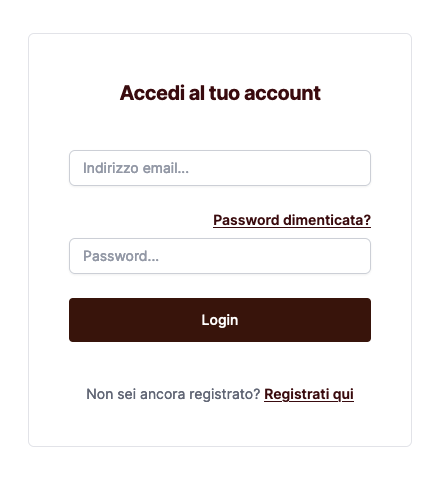
\includegraphics[width=0.3\linewidth]{img/form_login.png}
    \caption{Form login}
    \label{fig:form_login}
\end{figure}
In tutti e due i casi, comparirà una pagina nella quale verrà richiesto all'utente l'inserimento delle sue informazioni per potersi registrare; in particolare i campi richiesti sono: 
\begin{itemize}
    \item \textbf{email}: un'email valida che rispetta la formattazione xxx@yyy.zzz;
    \item \textbf{nome}: il nome dell'utente;
    \item \textbf{cognome}: il cognome dell'utente;
    \item \textbf{password}: una password valida.
\end{itemize}

\begin{figure}[H]
    \centering
    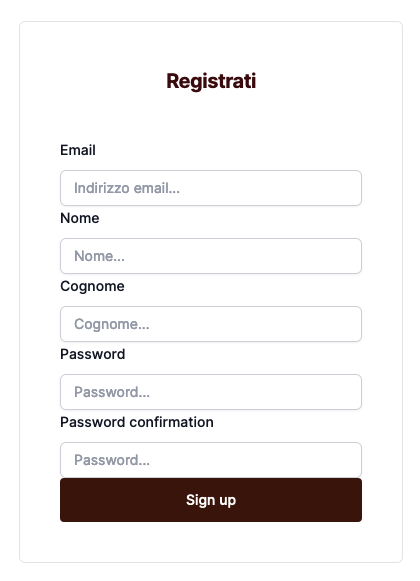
\includegraphics[width=0.4\linewidth]{img/schermata_registrazione.png}
    \caption{Form registrazione}
    \label{fig:form_signup}
\end{figure}

\subsubsection{Istruzioni per il login}
Per poter effettuare il login, cliccare sul pulsante \emph{login} nell'Header in alto a destra, oppure quello nella sezione "utente" nella home page.
\begin{figure}[H]
    \centering
    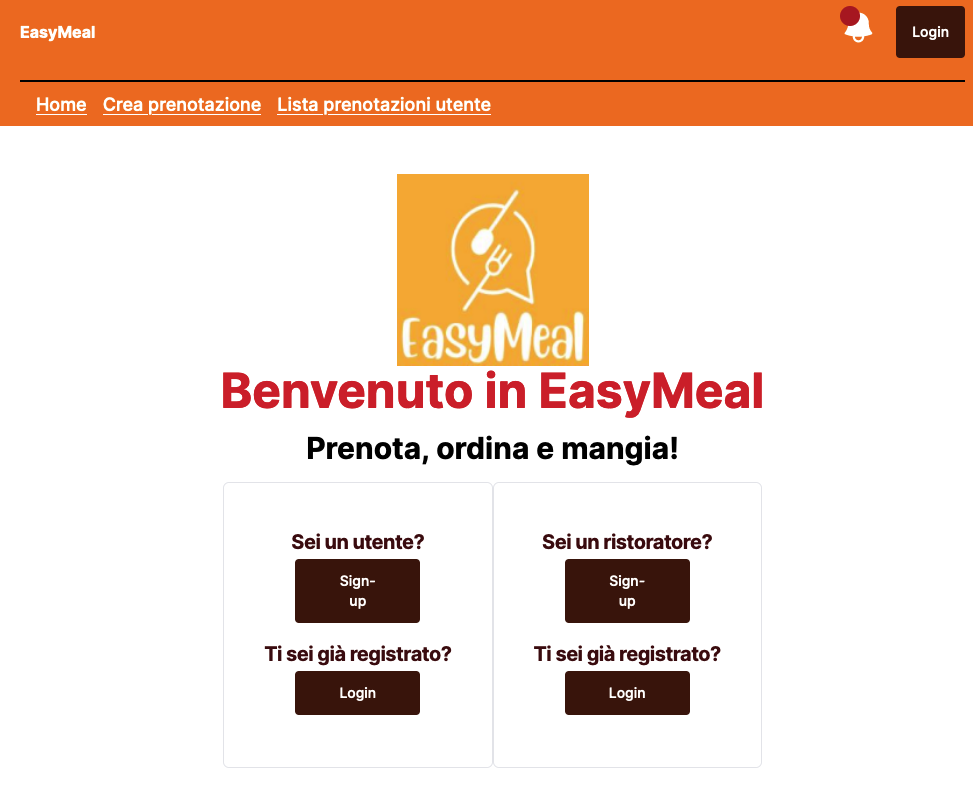
\includegraphics[width=0.6\linewidth]{img/inizio_login.png}
    \caption{Schermata home page}
    \label{fig:form_signup}
\end{figure}

Comparirà poi il seguente form, nel quale si chiede l'inserimento delle credenziali con le quali ci si è registrati nel $\textit{sistema}_G$; in particolare vengono richieste email e password.

\begin{figure}[H]
    \centering
    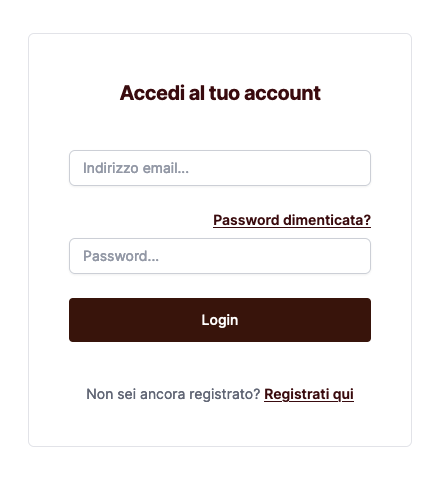
\includegraphics[width=0.3\linewidth]{img/form_login.png}
    \caption{Form login}
    \label{fig:form_login}
\end{figure}

\newpage
\subsubsection{Istruzioni per prenotare}
Dopo aver effettuato il login, l'utente si ritroverà nella pagina per la ricerca del ristorante, la quale è accessibile anche cliccando il link "\emph{Crea prenotazione}" presente nell'Header.
\begin{figure}[H]
    \centering
    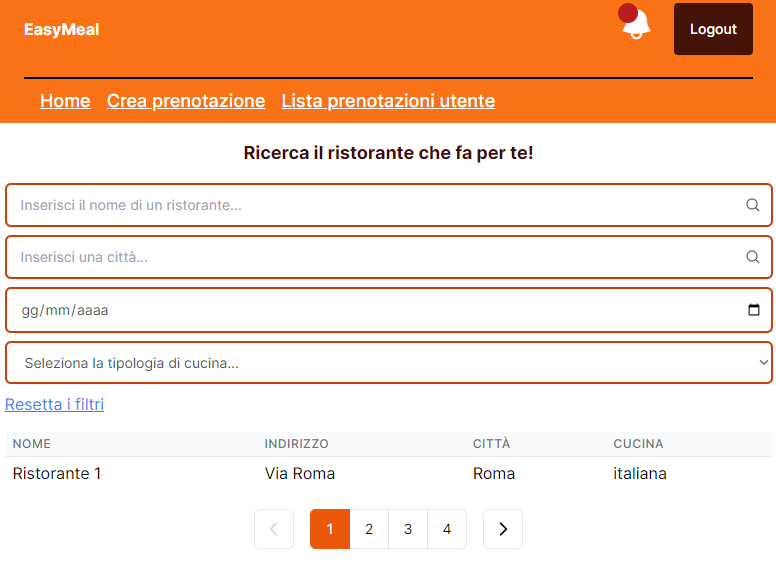
\includegraphics[width=0.6\linewidth]{img/ricerca_ristorante.png}
    \caption{Pagina per la ricerca del ristorante}
    \label{fig:ricerca_ristorante}
\end{figure}
Nella pagina sono presenti i seguenti filtri di ricerca:
\begin{itemize}
    \item \textbf{Nome ristorante}: in questo campo si inserisce il nome del ristorante che si vuole cercare;
    \item \textbf{Città}: in questo campo si inserisce il nome della città in cui si vuole trovare il ristorante;
    \item \textbf{Data}: in questo campo si inserisce la data in cui si ha intenzione di prenotare, così da individuare i ristoranti aperti quel giorno;
    \item \textbf{Tipologia cucina}: in questo campo si inserisce la tipologia della cucina.
\end{itemize}
Infine, è possibile resettare i filtri di ricerca, premendo sul link "Resetta i filtri".
\begin{figure}[H]
    \centering
    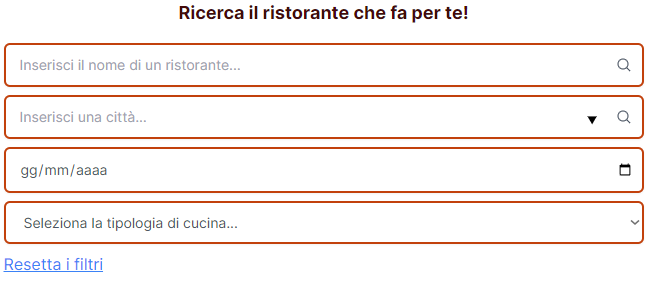
\includegraphics[width=0.6\linewidth]{img/form_ricerca.png}
    \caption{Form per la ricerca del ristorante}
    \label{fig:form_ricerca}
\end{figure}
Sotto il form di ricerca è presente la lista dei ristoranti che rispettano i parametri inseriti precedentemente. Ognuno di questi presenterà il nome, l'indirizzo, la città e la tipologia della cucina. Inoltre, è presente la funzionalità di paginazione, la quale permette all'utente di spostarsi in pagine successive o precedenti, nel caso in cui siano presenti più ristoranti che rispettano i filtri di ricerca. La pagina caricherà solo un certo numero di ristoranti, quindi per visualizzare ulteriori ristoranti, sarà necessario cliccare sul numero della pagina che si vuole raggiungere o spostarsi cliccando le frecce.
\begin{figure}[H]
    \centering
    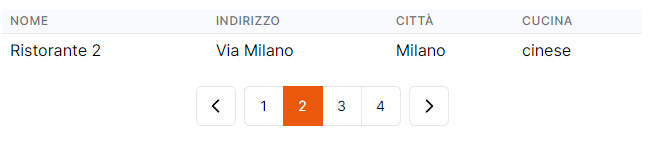
\includegraphics[width=0.6\linewidth]{img/lista_e_pagination.png}
    \caption{Elenco ristoranti e paginazione}
    \label{fig:lista_e_pagination}
\end{figure}
Cliccando sul nome del ristorante si accederà alla pagina di $\textit{prenotazione}_G$.

Nella metà superiore della pagina si visualizzeranno un'immagine del ristorante, le informazioni del ristorante e il menù.
\begin{figure}[H]
    \centering
    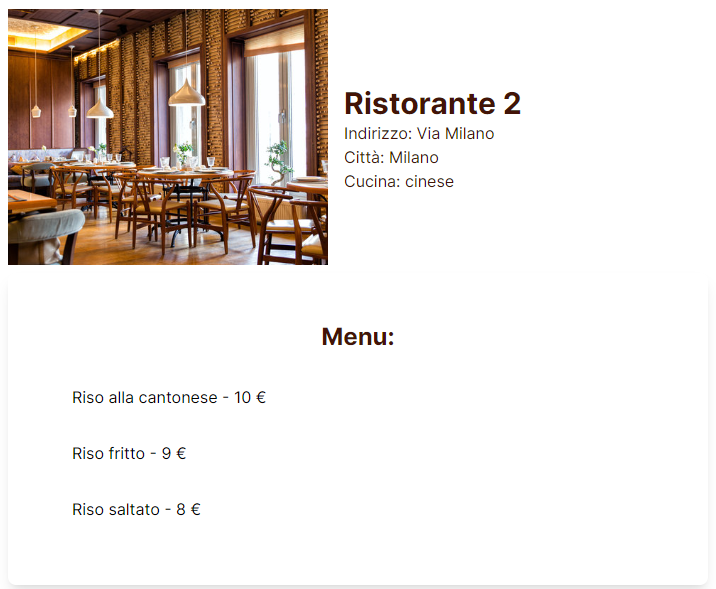
\includegraphics[width=0.6\linewidth]{img/prenotazione_info.png}
    \caption{Info ristorante e menù}
    \label{fig:prenotazione_info}
\end{figure}
Mentre, nella parte inferiore della pagina sarà presente il form per effettuare la $\textit{prenotazione}_G$. Qui l'utente dovrà inserire una data, l'orario di arrivo al ristorante e il numero di persone. Una volta inseriti questi dati per procedere si deve cliccare il tasto "\emph{prenota}".
\begin{figure}[H]
    \centering
    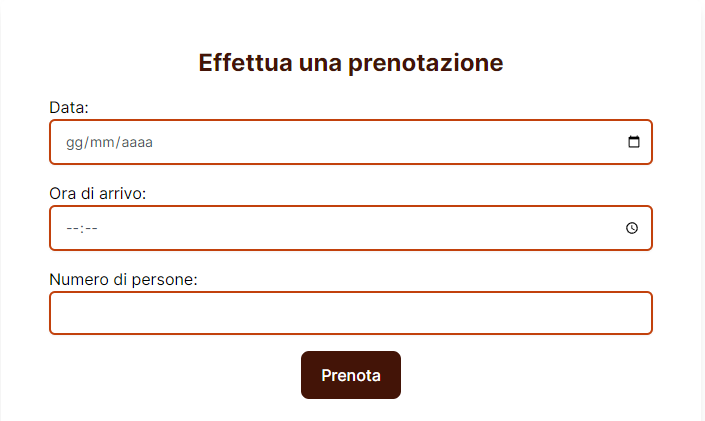
\includegraphics[width=0.6\linewidth]{img/prenotazione_form.png}
    \caption{Form prenotazione}
    \label{fig:prenotazione_form}
\end{figure}
Successivamente, l'utente si ritroverà nella pagina "\emph{lista prenotazioni}", in cui sarà presente la $\textit{prenotazione}_G$ appena fatta, nello stato "in attesa di conferma".
\begin{figure}[H]
    \centering
    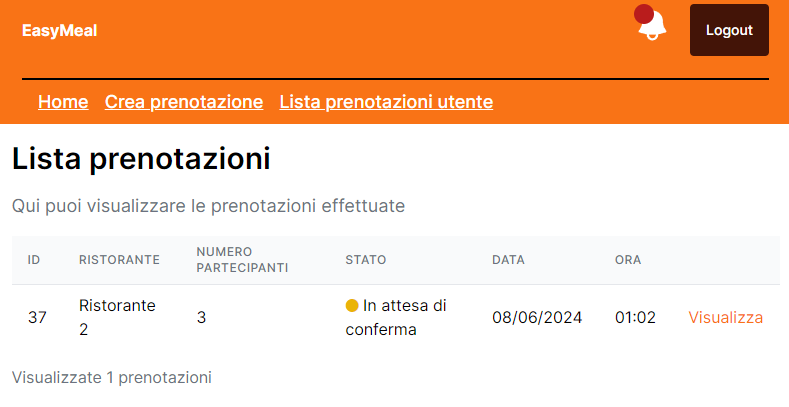
\includegraphics[width=0.6\linewidth]{img/lista_prenotazioni_post_prenotazione.png}
    \caption{Lista prenotazione con la prenotazione in stato "in attesa di conferma"}
    \label{fig:lista_prenotazioni_post_prenotazione}
\end{figure}

\newpage
\subsubsection{Istruzioni per ordinare}
Dopo che una $\textit{prenotazione}_G$ in un ristorante è stata accettata da un amministratore, l'utente che ha già effettuato il login può accedere alla schermata di $\textit{ordinazione}_G$, cliccando prima su "\emph{lista prenotazioni utente}" nell'Header della pagina , poi cliccando sul tasto "\emph{Visualizza}" della $\textit{prenotazione}_G$ accettata: 
\begin{figure}[H]
    \centering
    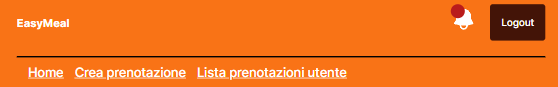
\includegraphics[width=0.6\linewidth]{img/header_utente.png}
    \caption{Header utente}
    \label{fig:header_utente}
\end{figure}
\begin{figure}[H]
    \centering
    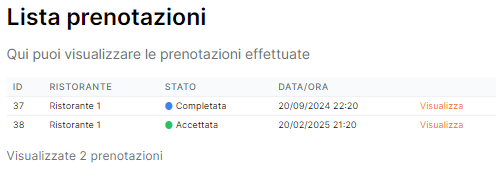
\includegraphics[width=0.6\linewidth]{img/lista_prenotazioni_utente.PNG}
    \caption{Lista prenotazioni utente}
    \label{fig:Lista prenotazioni utente}
\end{figure}
e infine cliccando sul bottone "\emph{Vai all'ordinazione}" posto in mezzo alla pagina:
\begin{figure}[H]
    \centering
    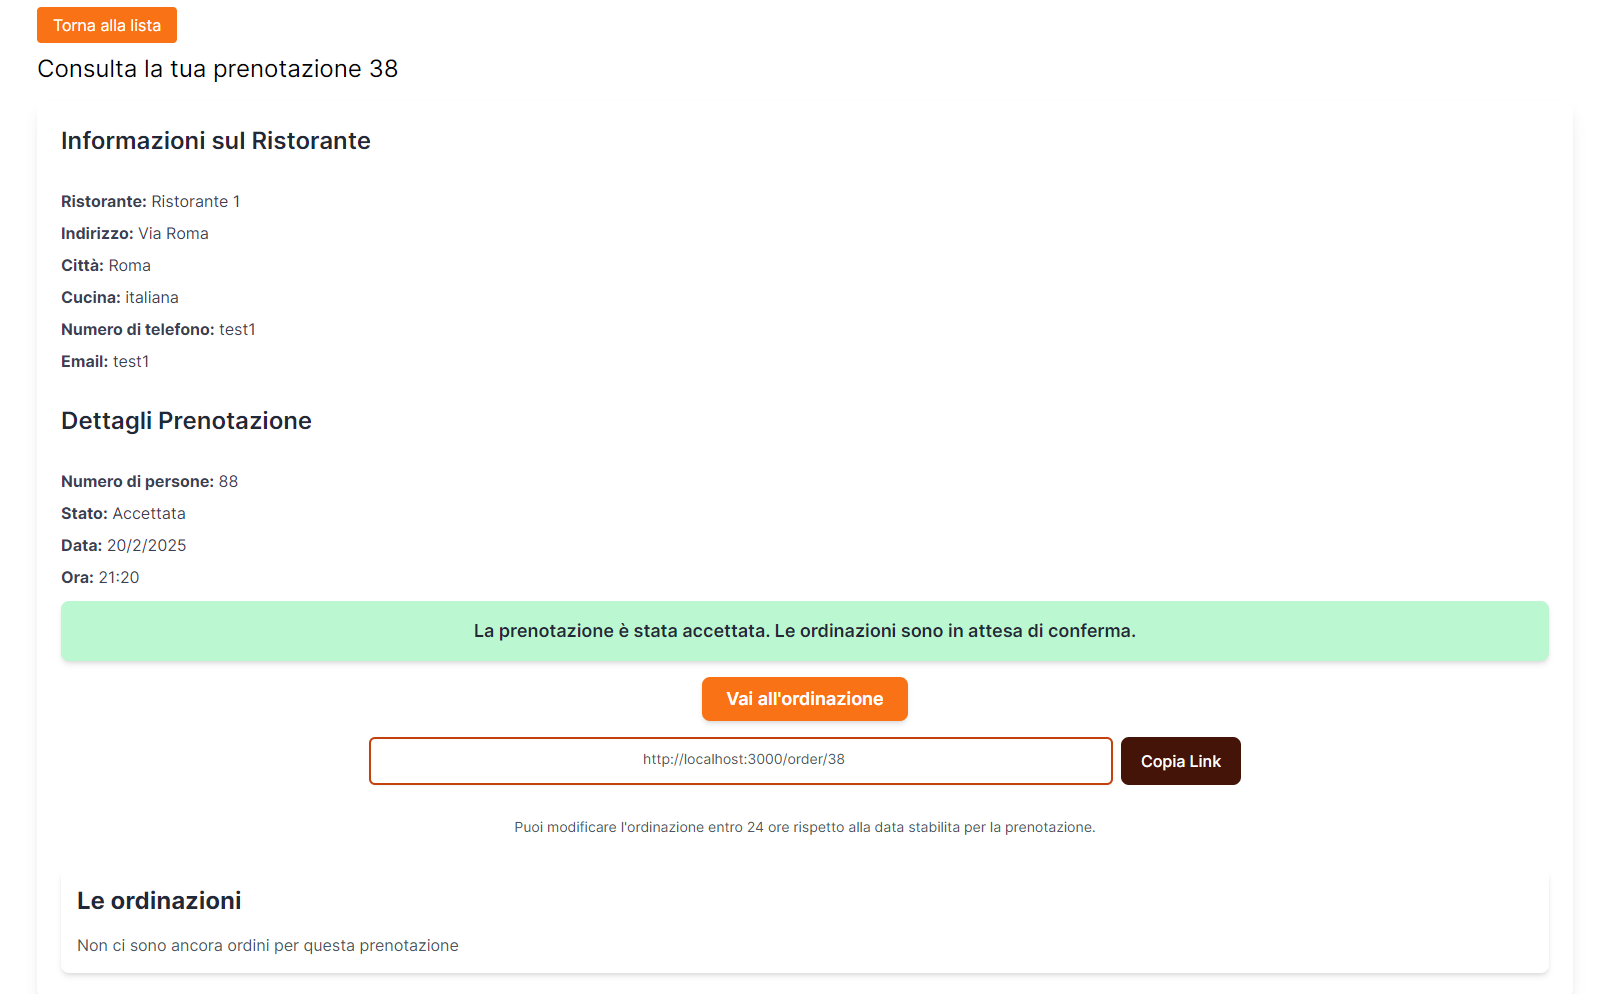
\includegraphics[width=0.75\linewidth]{img/dettaglio_prenotazione.PNG}
    \caption{Singola prenotazione}
    \label{fig:Singola prenotazione}
\end{figure}
 Si noti che se la $\textit{prenotazione}_G$ comprende più persone, esiste un link sotto il bottone "\emph{Vai all'$\textit{ordinazione}_G$}" che se usato da altri partecipanti permetterà a loro di effettuare \emph{l'$\textit{ordinazione}_G$ collaborativa}.
\\ Ora si possono ordinare i pasti che compaiono a schermo, con i dovuti pulsanti per aggiungere o rimuovere piatti alla $\textit{prenotazione}_G$.
\\Nel caso dell'$\textit{ordinazione}_G$ collaborativa, gli utenti con altri account che si collegano all'$\textit{ordinazione}_G$ tramite il link, modificheranno contemporaneamente le quantità di piatti da includere nell'$\textit{ordinazione}_G$ in maniera sincrona:
\begin{figure}[H]
    \centering
    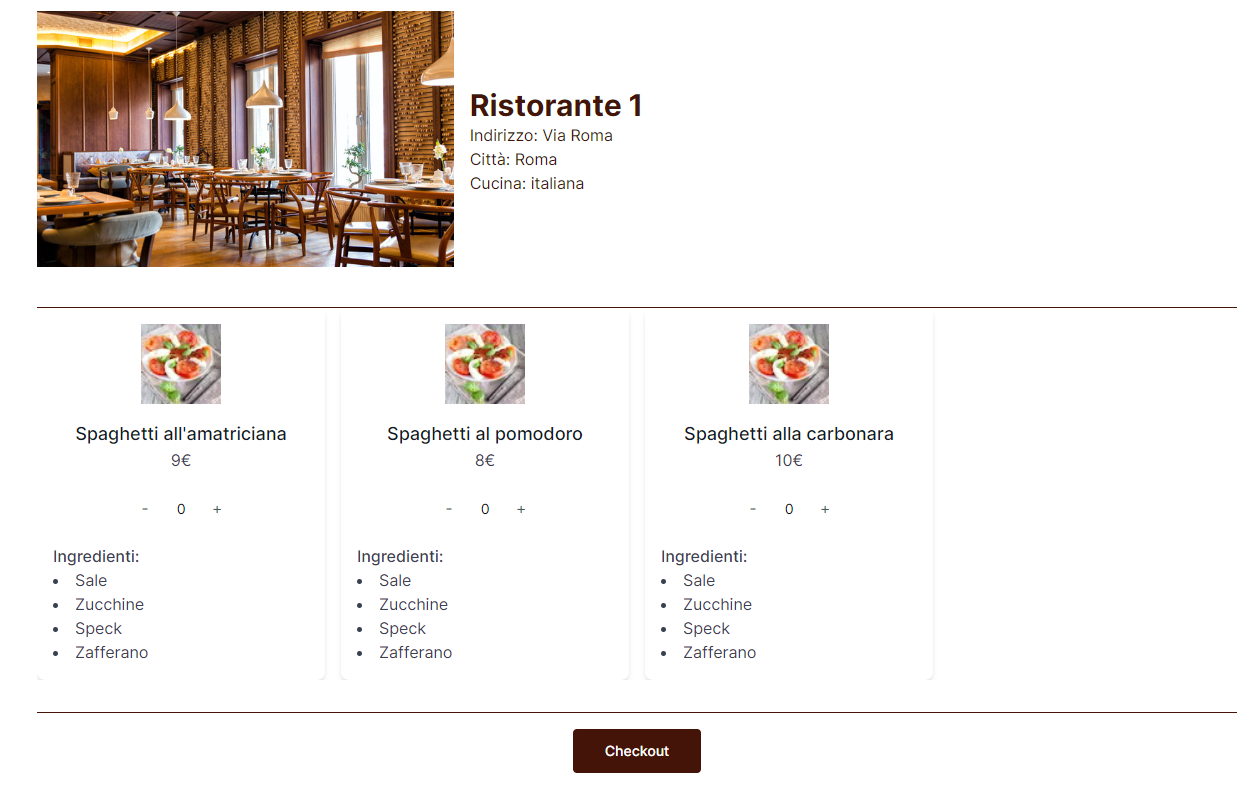
\includegraphics[width=0.7\linewidth]{img/ordinazione_ristorante.PNG}
    \caption{Ordinazione}
    \label{fig:Ordinazione}
\end{figure}
Cliccando su pulsante in basso "\emph{Checkout}" si accede all'ultima pagina dell'$\textit{ordinazione}_G$, che permette di aggiungere o togliere ingredienti per ogni piatto e scegliere il metodo di pagamento:
\begin{figure}[H]
    \centering
    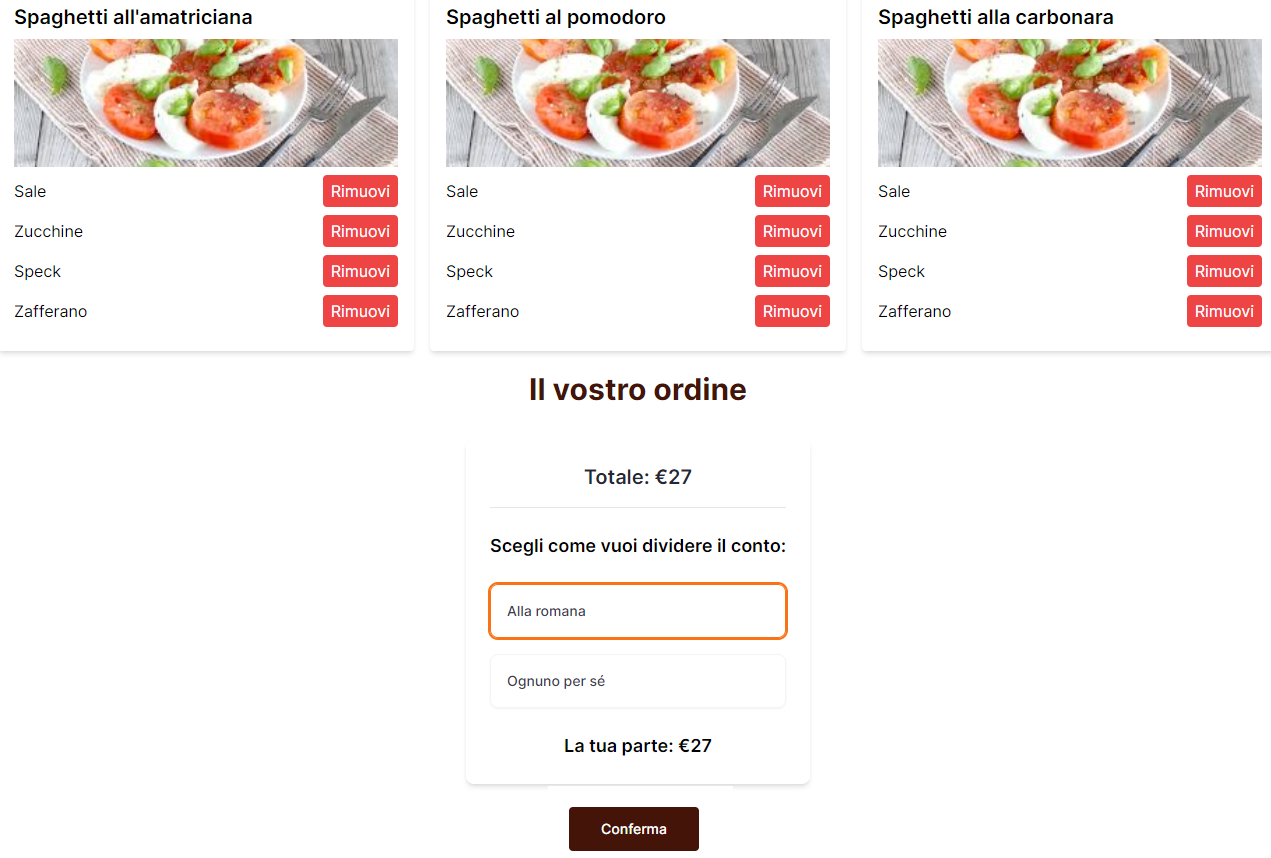
\includegraphics[width=0.7\linewidth]{img/checkout.PNG}
    \caption{Checkout}
    \label{fig:checkout}
\end{figure}
Cliccando sul pulsante "\emph{Conferma}" in fondo alla pagina, si viene reindirizzati alla pagina di dettaglio della $\textit{prenotazione}_G$, che ora informa che le ordinazioni sono state confermate e che si è in attesa del pagamento.
\newpage
\subsubsection{Istruzioni per il pagamento}
Una volta effettuato l'ordine si verrà rimandati direttamente ai dettagli della $\textit{prenotazione}_G$. Pagina eventualmente raggiungibile cliccando su "Lista prenotazioni utente" nell'Header e cliccando "visualizza" sull'ordine desiderato (in questo caso quello con lo stato "da pagare").
\begin{figure}[H]
    \centering
    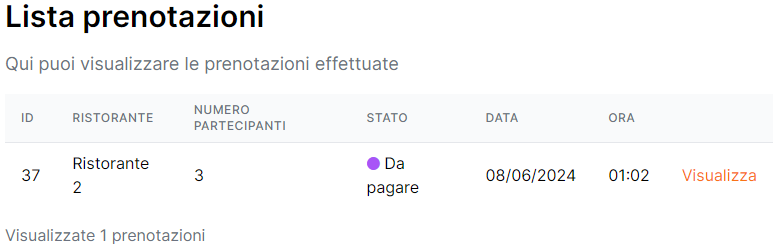
\includegraphics[width=0.6\linewidth]{img/stato_to_pay.png}
    \caption{Pagina con i dettagli della prenotazione nello stato "to pay"}
    \label{fig:stato_to_pay}
\end{figure}
Nei dettagli della $\textit{prenotazione}_G$, sarà possibile vedere innanzitutto le informazioni del ristorante e della $\textit{prenotazione}_G$ stessa.
\begin{figure}[H]
    \centering
    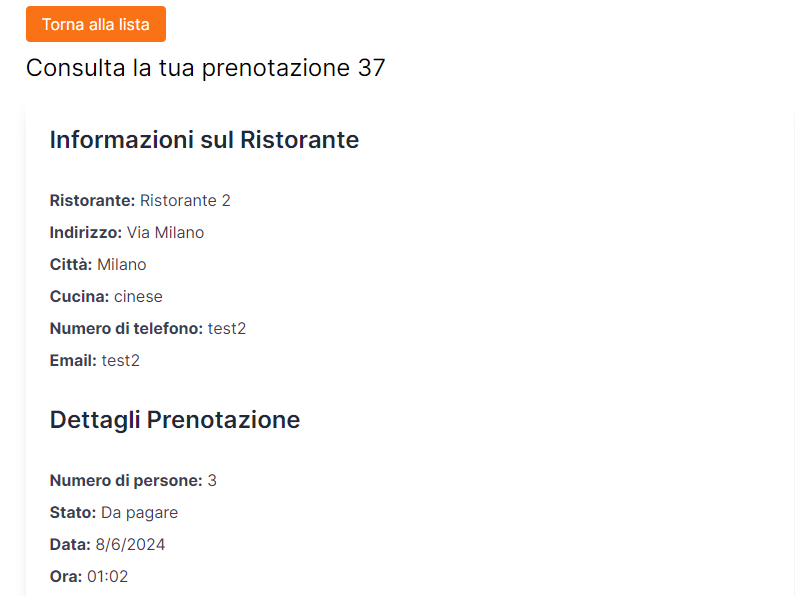
\includegraphics[width=0.6\linewidth]{img/dettagli_prenotazione_to_pay_superiore.png}
    \caption{Parte superiore della pagina con i dettagli della prenotazione nello stato "da pagare"}
    \label{fig:dettagli_prenotazione_to_pay_superiore}
\end{figure}

Invece, in fondo alla pagina sarà possibile vedere un riepilogo di quello che è stato ordinato e da chi.
\begin{figure}[H]
    \centering
    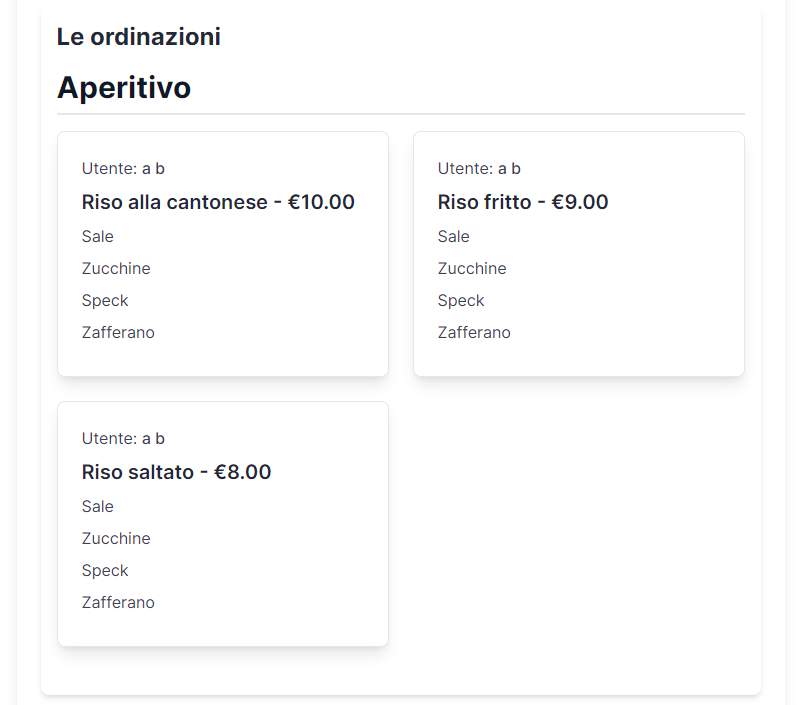
\includegraphics[width=0.6\linewidth]{img/dettagli_prenotazione_to_pay_inferiore.png}
    \caption{Parte inferiore della pagina con i dettagli della prenotazione nello stato "da pagare"}
    \label{fig:dettagli_prenotazione_to_pay_inferiore}
\end{figure}
Infine, a metà pagina invece ci sono le informazioni riguardanti il pagamento. Qui si può vedere chi ha partecipato all'$\textit{ordinazione}_G$, se la propria quota è stata pagata, la cifra che l'utente deve pagare rispetto al totale, la modalità della divisione del conto e l'effettivo tasto "Paga la tua parte", che permette di saldare la propria parte di conto.
\begin{figure}[H]
    \centering
    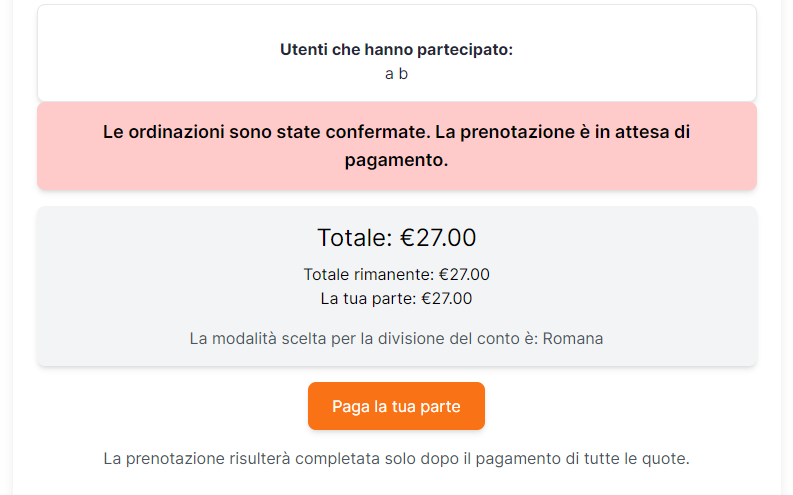
\includegraphics[width=0.6\linewidth]{img/paga.png}
    \caption{Parte centrale della pagina con i dettagli della prenotazione nello stato "da pagare"}
    \label{fig:paga}
\end{figure}
Nel caso in cui la $\textit{prenotazione}_G$ è stata pagata da tutti gli utenti che hanno partecipato, allora uscirà il seguente messaggio nei dettagli della $\textit{prenotazione}_G$.
\begin{figure}[H]
    \centering
    
\includegraphics[width=0.6\linewidth]{img/prenotazione_pagata_e_completata.png}
    \caption{Messaggio di quando la prenotazione è stata pagata e completata}
    \label{fig:prenotazione_pagata_e_completata}
\end{figure}
Invece, se la $\textit{prenotazione}_G$ non è stata pagata da tutti uscirà il totale rimanente da pagare e il seguente messaggio.
\begin{figure}[H]
    \centering
    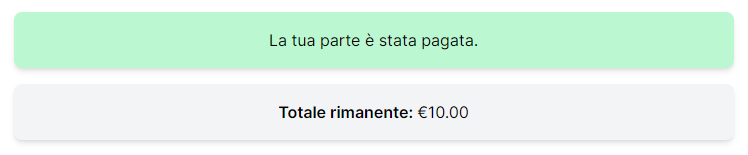
\includegraphics[width=0.6\linewidth]{img/pagata_parte.png}
    \caption{Messaggio di quando la propria parte è stata pagata}
    \label{fig:pagata_parte}
\end{figure}

\subsubsection{Visualizzazione delle prenotazioni effettuate}
Tramite l'apposito link posto nell'Header, un utente base può andare a visualizzare tutte le prenotazioni da lui effettuate nel corso del suo utilizzo di \textit{EasyMeal}. 
\begin{figure}[H]
    \centering
    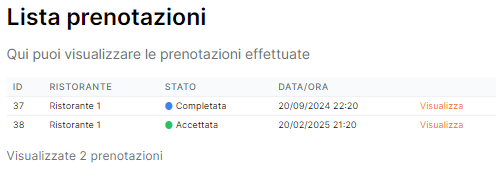
\includegraphics[width=0.6\linewidth]{img/lista_prenotazioni_utente.PNG}
    \caption{Visualizzazione della lista delle prenotazioni di un utente base}
\end{figure}
Per ogni $\textit{prenotazione}_G$, è possibile visualizzare direttamente dall'elenco: 
\begin{itemize}
    \item \textbf{ID}: parametro identificativo univoco di una determinata $\textit{prenotazione}_G$;
    \item \textbf{RISTORANTE}: nome del ristorante presso il quale è stata effettuata la $\textit{prenotazione}_G$ in esame; 
    \item \textbf{STATO}: stato di una determinata $\textit{prenotazione}_G$. Esso può essere: 
    \begin{itemize}
        \item \textbf{In attesa di conferma}: una $\textit{prenotazione}_G$ effettuata ma ancora non confermata da parte dell'amministratore; 
        \item \textbf{Accettata}: una $\textit{prenotazione}_G$ accettata da parte dell'amministratore del ristorante in esame ma di cui non è stata ancora fatta la relativa $\textit{ordinazione}_G$; 
        \item \textbf{Da pagare}: una $\textit{prenotazione}_G$ di cui è stata fatta l'$\textit{ordinazione}_G$ ma per cui manca ancora il pagamento; 
        \item \textbf{Completata}: una $\textit{prenotazione}_G$ andata a buon fine.
        \item \textbf{Rifiutata}: una $\textit{prenotazione}_G$ che è stata rifiutata da parte dell'amministratore del ristorante in esame. 
    \end{itemize}
    \item \textbf{DATA/ORA}: la data e l'ora richieste relativamente alla $\textit{prenotazione}_G$ in esame. 
\end{itemize}
E' possibile poi andare nel dettaglio di una determinata $\textit{prenotazione}_G$, schiacciando sul link "Visualizza" presente a fianco di ogni voce della tabella delle prenotazioni. 
\begin{figure}[H]
    \centering
    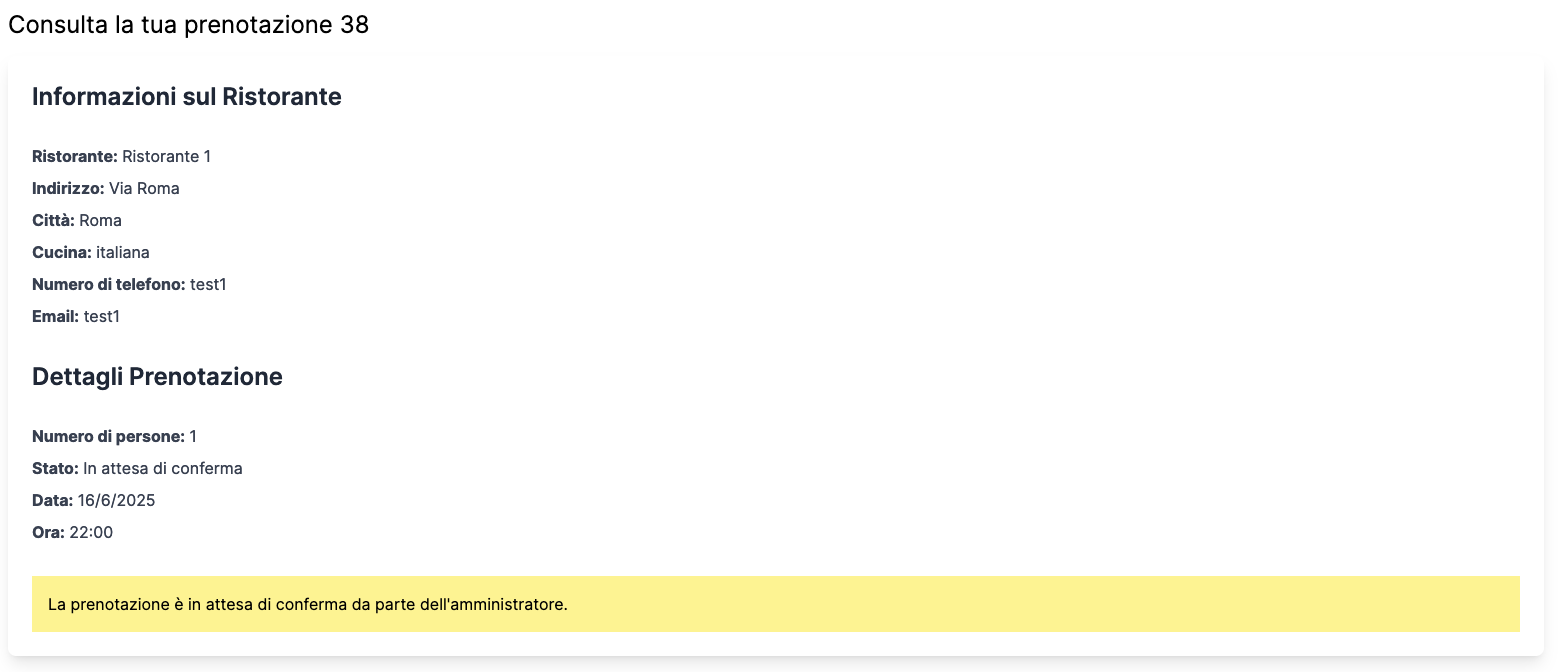
\includegraphics[width=0.6\linewidth]{img/dettaglio_prenotazione_user.png}
    \caption{Visualizzazione del dettaglio di una determinata prenotazione}
\end{figure}

\subsubsection{Notifiche}
\textit{Easy Meal} possiede un $\textit{sistema}_G$ di notifiche, tramite le quali un utente base può essere informato dello stato di avanzamento di una sua $\textit{prenotazione}_G$. \\
Le notifiche possono apparire come \textit{alerts} del browser, nel caso in cui l'utente interessato dalla notifica stessa sia online nel momento della ricezione della notifica, oppure possono sempre essere visualizzate accedendo alla pagina "Notifiche" tramite l'apposito pulsante posto nell'Header. 
\begin{figure}[H]
    \centering
    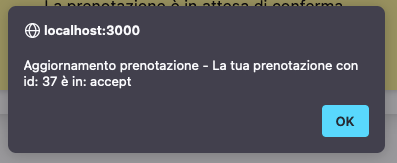
\includegraphics[width=0.4\linewidth]{img/notica_browser.png}
    \caption{Apparizione di una notifica tramite messaggio del browser su Firefox}
\end{figure}
\begin{figure}[H]
    \centering
    
\includegraphics[width=0.8\linewidth]{img/notifica_pagina.png}
    \caption{Visualizzazione di una modifica nella pagina "Notifiche"}
\end{figure}
Durante il $\textit{processo}_G$ di creazione di una $\textit{prenotazione}_G$, come utente si riceveranno varie notifiche relative allo stato della stessa: 
\begin{itemize}
    \item \textbf{Notifica per quando una $\textit{prenotazione}_G$ è accettata}: L'utente, una volta piazzata una $\textit{prenotazione}_G$, riceverà una notifica nel momento in cui l'amministratore del ristorante per cui ha scelto di prenotare avrà accettato la stessa. 
    \item \textbf{Notifica per quando una $\textit{prenotazione}_G$ è confermata}: L'utente, una volta fatta l'$\textit{ordinazione}_G$, riceverà una notifica nel momento in cui l'amministratore conferma la disponibilità dei piatti scelti dall'utente e segnerà la $\textit{prenotazione}_G$ come confermata. A questo punto, l'utente può procedere con il pagamento. 
\end{itemize}


\newpage
\subsection{Amministratore}

\subsubsection{Istruzioni per la registrazione}

Una volta arrivati nella pagina iniziale del sito, ci si può registrare come utente normale cliccando il pulsante registrati sotto la voce ristorante.

\begin{figure}[H]
    \centering
    
\includegraphics[width=0.5\linewidth]{img/schermata_iniziale.png}
    \caption{Form login}
    \label{fig:schermata_iniziale}
\end{figure}

Comparirà una pagina nella quale verrà richiesto all'utente l'inserimento delle sue informazioni per poter registrare lui e il suo ristorante all'interno del $\textit{sistema}_G$; in particolare i campi richiesti sono: 

\begin{itemize}
    \item \textbf{email}: un'email valida rispetta la formattazione xxx@yyy.zzz;
    \item \textbf{nome}: il nome dell'utente;
    \item \textbf{cognome}: il cognome dell'utente;
    \item \textbf{nome del ristorante}: il nome del ristorante gestito dall'utente.
    \item \textbf{città}: la città nella quale risiede il ristorante.
    \item \textbf{indirizzo}: l'indirizzo del locale.
    \item \textbf{descrizione}: una breve descrizione del ristorante.
    \item \textbf{orari}: una lista di giorni che, se selezionati, portano l'utente a specificare sia l'orario di apertura che di chiusura del ristorante in un determinato giorno.
    \item \textbf{coperti}: il numero di tavoli che il ristorante mette a disposizione.
    \item \textbf{email ristorante}: l'email associata al ristorante.
    \item \textbf{tipologica di cucina}: la tipologia di cucina che il ristorante offre.
    \item \textbf{password}: una password valida.
\end{itemize}

\begin{figure}[H]
    \centering
    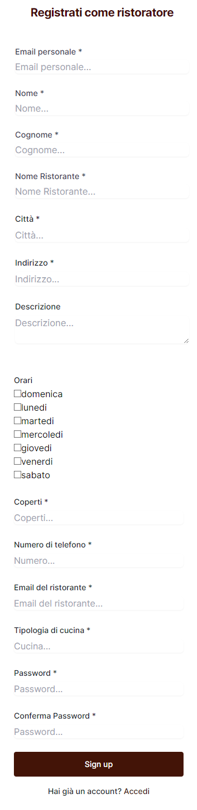
\includegraphics[width=0.25\linewidth]{img/sign-up-admin.png}
    \caption{Form registrazione ristoratore}
    \label{fig:form_signup}
\end{figure}

\subsubsection{Istruzioni per il login}

Per poter effettuare il login, cliccare sul pulsante \emph{login} nell'Header in alto a destra, oppure il pulsante login nel form "ristoratore" nella home page.

\begin{figure}[H]
    \centering
    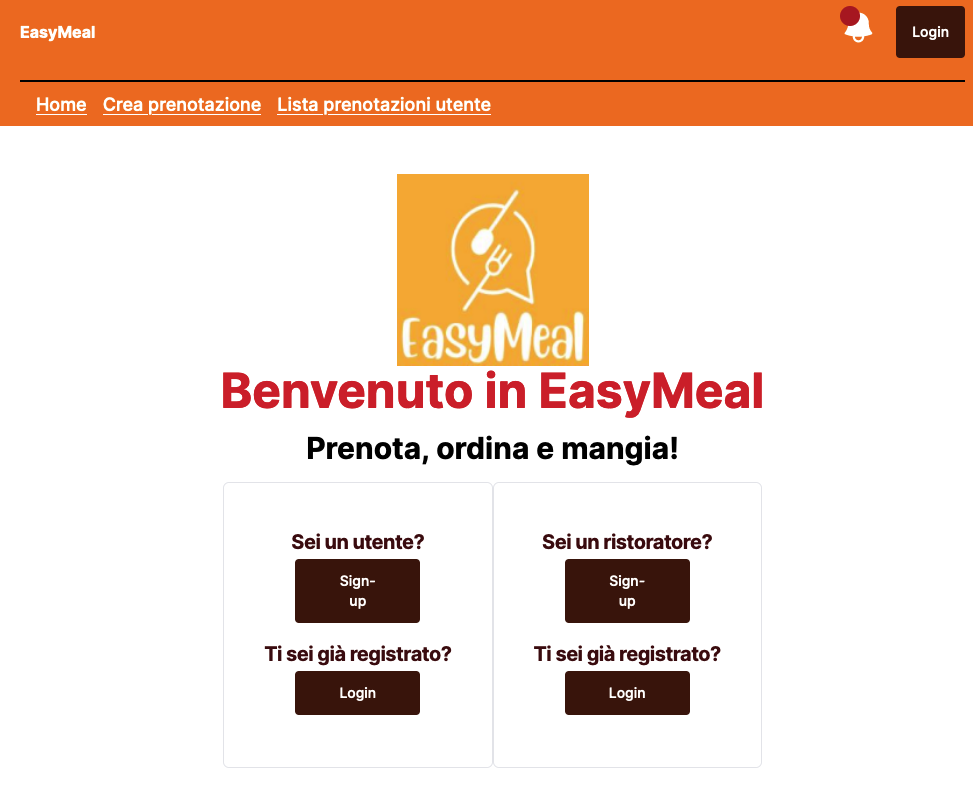
\includegraphics[width=0.6\linewidth]{img/inizio_login.png}
    \caption{Schermata iniziale}
    \label{fig:form_signup}
\end{figure}

Comparirà poi il seguente form, nel quale si chiede l'inserimento delle credenziali con le quali ci si è registrati nel $\textit{sistema}_G$; in particolare vengono richieste email e password.

\begin{figure}[H]
    \centering
    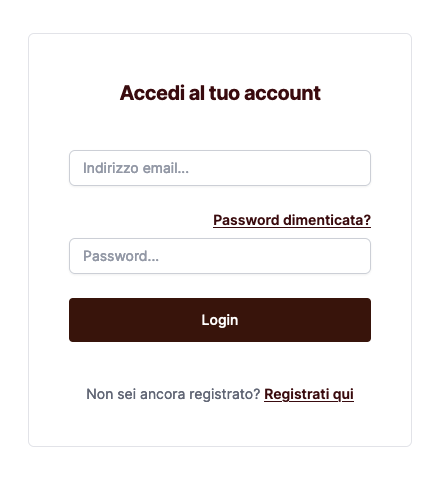
\includegraphics[width=0.3\linewidth]{img/form_login.png}
    \caption{Form login}
    \label{fig:form_login}
\end{figure}

\newpage
\subsubsection{Accettare o rifiutare prenotazioni}
Un admin che ha già effettuato il login, può accedere alla schermata di accettazione o rifiuto di una $\textit{prenotazione}_G$, cliccando prima su "\emph{Lista prenotazioni ristorante}", poi cliccando sul tasto "Visualizza" della $\textit{prenotazione}_G$ da gestire:
\begin{figure}[H]
    \centering
    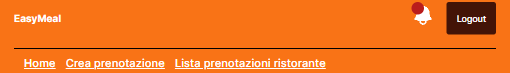
\includegraphics[width=0.6\linewidth]{img/Header_admin.png}
    \caption{Header utente}
    \label{fig:Header utente}
\end{figure}
\begin{figure}[H]
    \centering
    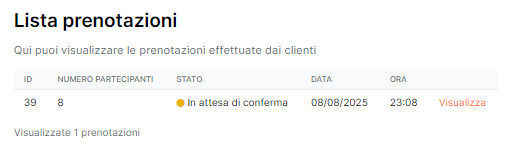
\includegraphics[width=0.6\linewidth]{img/lista_prenotazioni_admin.PNG}
    \caption{Lista prenotazioni Admin}
    \label{fig:Lista prenotazioni Admin}
\end{figure}

A questo punto, la schermata che verrà mostrata conterrà i dati della $\textit{prenotazione}_G$ in entrata con gli opportuni pulsati per l'accettazione ed il rifiuto della $\textit{prenotazione}_G$:
\begin{figure}[H]
    \centering
    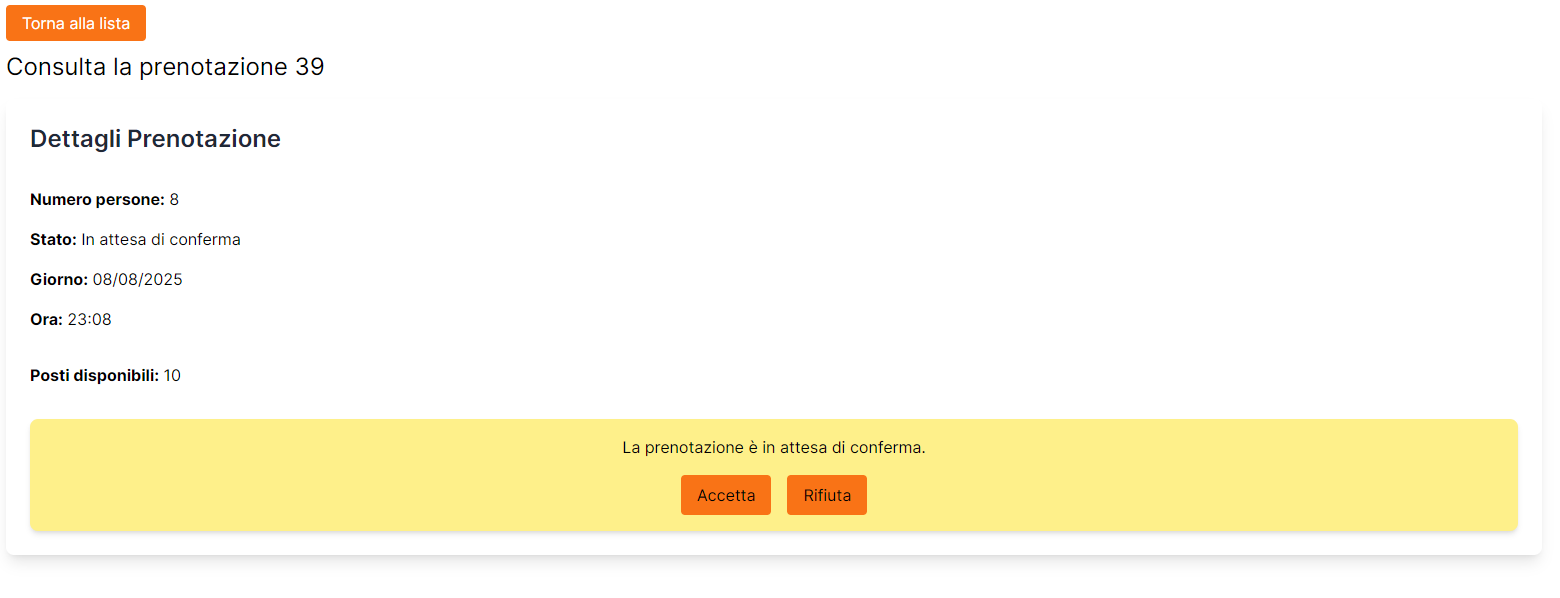
\includegraphics[width=0.6\linewidth]{img/menu_accettazione_rifiuto.PNG}
    \caption{Accettazione/Rifiuto prenotazione}
    \label{fig:Accettazione/Rifiuto prenotazione}
\end{figure}

\newpage
\paragraph{Prenotazione accettata}: \\
Se l'amministratore accetta la $\textit{prenotazione}_G$ con il tasto "\emph{Accetta}", verrà visualizzato un messaggio esplicativo dell'accettazione.
\begin{figure}[H]
    \centering
    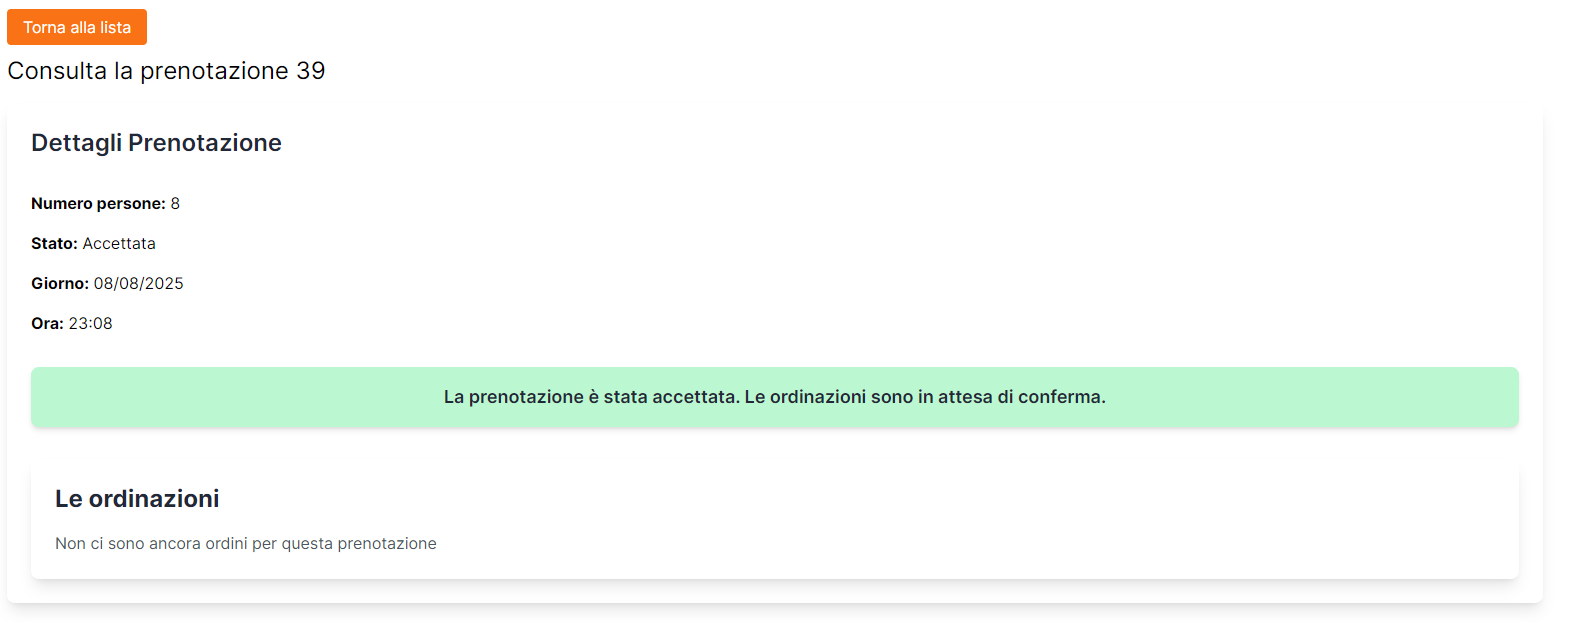
\includegraphics[width=0.75\linewidth]{img/accettazione_prenotazione.PNG}
    \caption{Accettazione prenotazione}
    \label{fig:Accettazione prenotazione}
\end{figure}

\paragraph{Prenotazione rifiutata}: \\
Se l'amministratore rifiuta la $\textit{prenotazione}_G$ con il tasto "\emph{Rifiuta}", verrà visualizzato un messaggio esplicativo del rifiuto.
\begin{figure}[H]
    \centering
    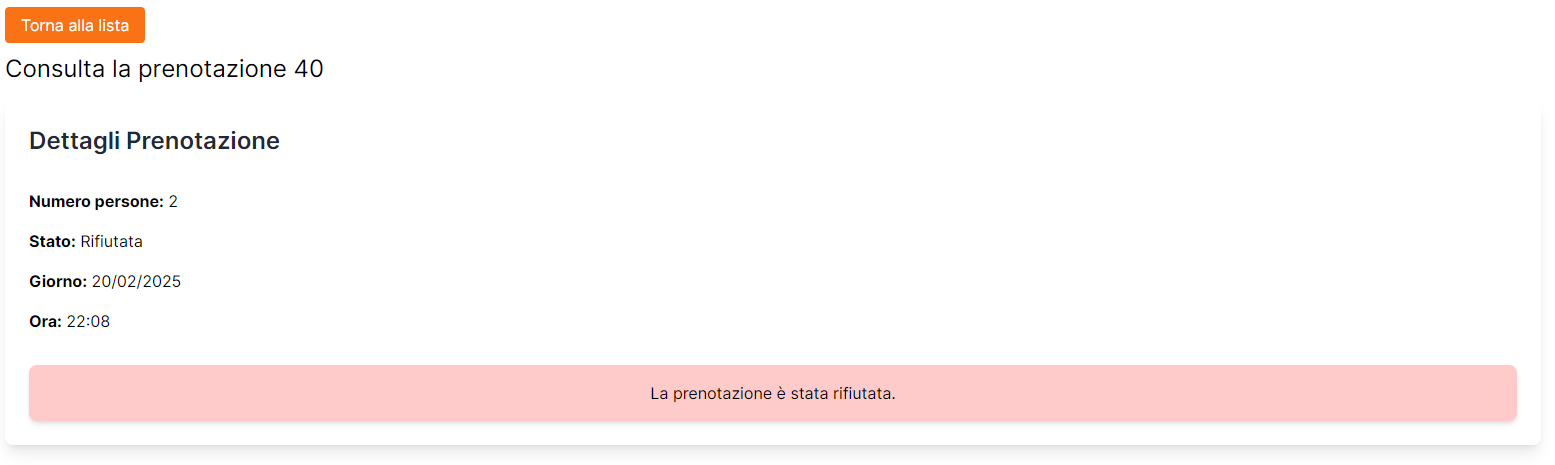
\includegraphics[width=0.75\linewidth]{img/rifiuto_prenotazione.PNG}
    \caption{Rifiuto prenotazione}
    \label{fig:Rifiuto prenotazione}
\end{figure}
Inoltre, in base alla decisione dell'amministratore, questo aggiornerà lo stato di una $\textit{prenotazione}_G$ all'intero della lista contenuta nella sezione "\emph{Lista prenotazioni ristorante}".
\begin{figure}[H]
    \centering
    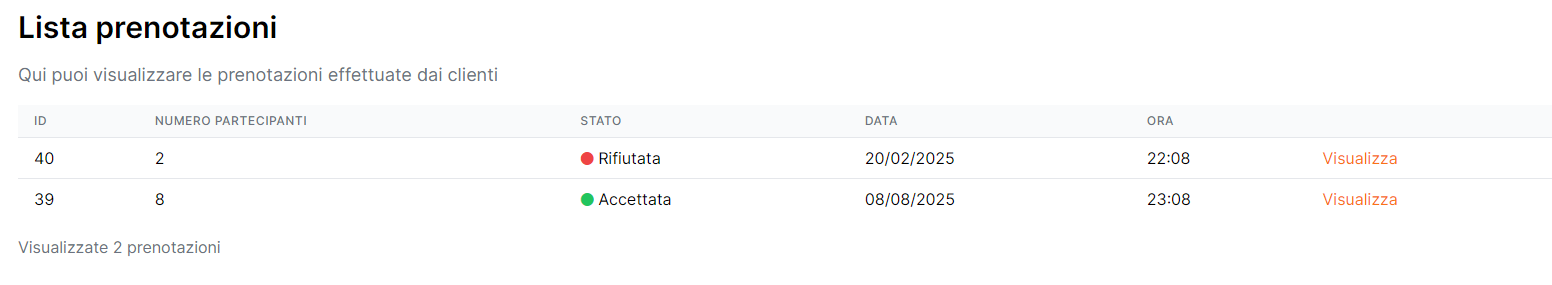
\includegraphics[width=0.85\linewidth]{img/stati_prenotazione.PNG}
    \caption{Stato prenotazioni}
    \label{fig:Stato prenotazioni}
\end{figure}

\newpage
\subsubsection{Visualizzazione delle prenotazioni ricevute}
Tramite l'apposito link posto nell'Header, un amministratore può andare a visualizzare tutte le prenotazioni ricevute per il suo ristorante nel corso del suo utilizzo di \textit{EasyMeal}. 
\begin{figure}[H]
    \centering
    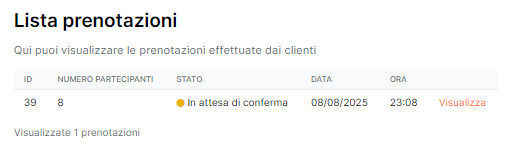
\includegraphics[width=0.6\linewidth]{img/lista_prenotazioni_admin.PNG}
    \caption{Visualizzazione della lista delle prenotazioni di un amministratore}
\end{figure}
Per ogni $\textit{prenotazione}_G$, è possibile visualizzare direttamente dall'elenco: 
\begin{itemize}
    \item \textbf{ID}: parametro identificativo univoco di una determinata $\textit{prenotazione}_G$;
    \item \textbf{RISTORANTE}: nome del ristorante presso il quale è stata effettuata la $\textit{prenotazione}_G$ in esame; 
    \item \textbf{STATO}: stato di una determinata $\textit{prenotazione}_G$. Esso può essere: 
    \begin{itemize}
        \item \textbf{In attesa di conferma}: una $\textit{prenotazione}_G$ effettuata ma ancora non confermata da parte dell'amministratore; 
        \item \textbf{Accettata}: una $\textit{prenotazione}_G$ accettata da parte dell'amministratore del ristorante in esame ma di cui non è stata ancora fatta la relativa $\textit{ordinazione}_G$; 
        \item \textbf{Da pagare}: una $\textit{prenotazione}_G$ di cui è stata fatta l'$\textit{ordinazione}_G$ ma per cui manca ancora il pagamento; 
        \item \textbf{Completata}: una $\textit{prenotazione}_G$ andata a buon fine.
        \item \textbf{Rifiutata}: una $\textit{prenotazione}_G$ che è stata rifiutata da parte dell'amministratore del ristorante in esame. 
    \end{itemize}
    \item \textbf{DATA/ORA}: la data e l'ora richieste relativamente alla $\textit{prenotazione}_G$ in esame. 
\end{itemize}
E' possibile poi andare nel dettaglio di una determinata $\textit{prenotazione}_G$, schiacciando sul link "Visualizza" presente a fianco di ogni voce della tabella delle prenotazioni. 
\begin{figure}[H]
    \centering
    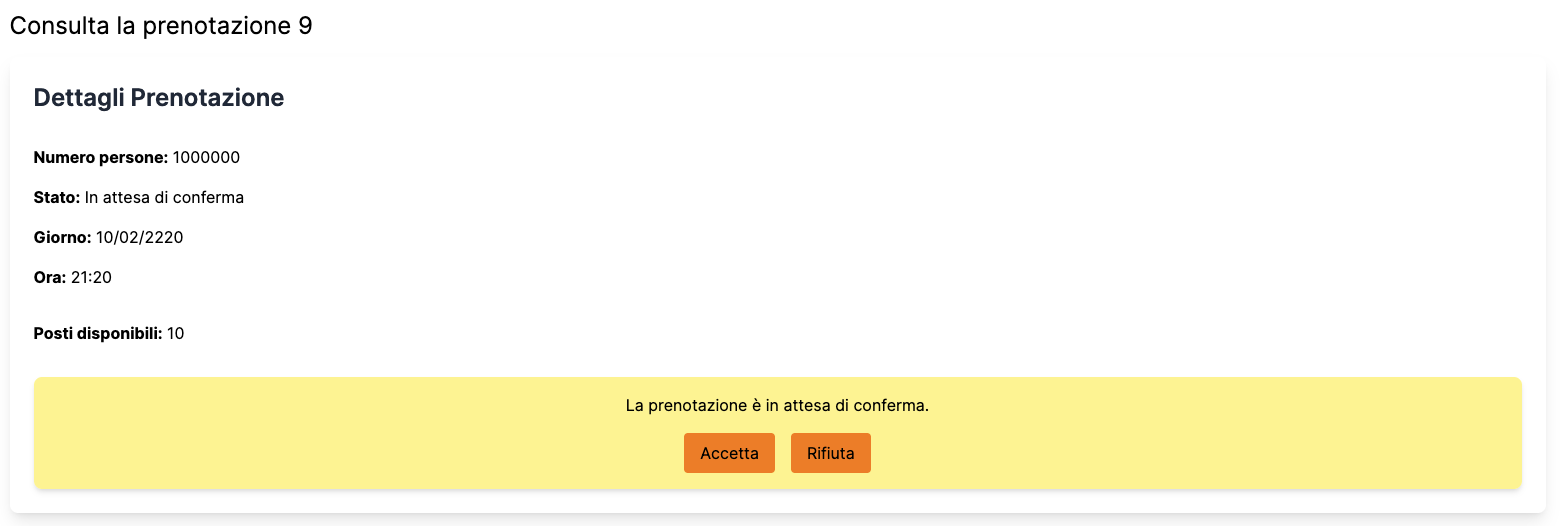
\includegraphics[width=0.6\linewidth]{img/dettaglio_prenotazione_admin.png}
    \caption{Visualizzazione del dettaglio di una determinata prenotazione}
\end{figure}
A seconda dello stato in cui si trova una determinata $\textit{prenotazione}_G$, tramite la pagina di visualizzazione dettagliata di una determinata $\textit{prenotazione}_G$ l'amministratore è in grado di compiere azioni relative alla stessa, tra cui accettarla o rifiutarla. 

\subsubsection{Notifiche}
\textit{Easy Meal} possiede un $\textit{sistema}_G$ di notifiche, tramite le quali un amministratore può essere informato dello stato di avanzamento di una $\textit{prenotazione}_G$ effettuata da un utente base. \\
Le notifiche possono apparire come \textit{alerts} del browser, nel caso in cui l'amministratore interessato dalla notifica stessa sia online nel momento della ricezione della notifica, oppure possono sempre essere visualizzate accedendo alla pagina "Notifiche" tramite l'apposito pulsante posto nell'Header. 
\begin{figure}[H]
    \centering
    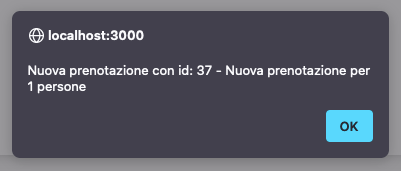
\includegraphics[width=0.4\linewidth]{img/notifica_browser_admin.png}
    \caption{Apparizione di una notifica tramite messaggio del browser su Firefox}
\end{figure}
\begin{figure}[H]
    \centering
    
\includegraphics[width=0.8\linewidth]{img/notifica_pagina_admin.png}
    \caption{Visualizzazione di una modifica nella pagina "Notifiche"}
\end{figure}
Durante il $\textit{processo}_G$ di creazione di una $\textit{prenotazione}_G$, come amministratore si riceveranno varie notifiche relative allo stato della stessa: 
\begin{itemize}
    \item \textbf{Notifica per quando è stata inserita una nuova $\textit{prenotazione}_G$}: L'amministratore di un determinato ristorante riceverà una notifica nel momento in cui un utente abbia richiesto di effettuare una $\textit{prenotazione}_G$ presso il suo ristorante. 
    \item \textbf{Notifica per quando è stata inserita l'$\textit{ordinazione}_G$}: L'amministratore riceverà una notifica nel momento in cui tutti gli utenti hanno terminato con l'inserimento dei piatti dell'$\textit{ordinazione}_G$ relativa a una $\textit{prenotazione}_G$ effettuata dagli stessi presso il ristorante dell'amministratore in esame. 
    \item \textbf{Notifica per quando è stata pagata una $\textit{prenotazione}_G$}: L'amministratore riceverà una notifica nel momento in cui il saldo relativo a una specifica $\textit{ordinazione}_G$ è stato pagato da parte dei partecipanti alla $\textit{prenotazione}_G$ stessa. 
\end{itemize}
\newpage

%Supporto Tecnico
\section{Supporto tecnico}
Per assistenza tecnica relativa all'utilizzo del prodotto $\textit{software}_G$ “\textit{EasyMeal}", viene fornito il seguente indirizzo email: 
\begin{center}
    \href{mailto:ramtastic6@gmail.com}{ramtastic6@gmail.com}
\end{center}
Per un servizio più efficiente, si è pregati di includere nel corpo dell'email una descrizione più completa possibile del problema riscontrato, insieme ad ogni possibile screenshot o dettaglio aggiuntivo che possano risultare utili alla risoluzione di quest'ultimo (frequenza, modalità di riproduzione del problema, etc.). \\
Si invita, inoltre, a descrivere eventuali passaggi già tentati per risolvere il problema, in modo che il team possa fornire un'assistenza più mirata.
\newpage

\end{document}